\documentclass[11pt,letterpaper]{article}


\usepackage{fullpage}
\usepackage[top=1cm, bottom=4.5cm, left=2.5cm, right=2.5cm]{geometry}
\usepackage{amsmath,amsthm,amsfonts,amssymb,amscd}
\usepackage{lastpage}
\usepackage{enumerate}
\usepackage{fancyhdr}
\usepackage{mathrsfs}
\usepackage{xcolor}
\usepackage{graphicx}
\usepackage{listings}
\usepackage{hyperref}
\usepackage{graphicx}
\usepackage{svg}
\usepackage{float}


\input defs.tex  %load E6602 macros

\title{{\LARGE \bf Design of a Rotational Flexure using Nonlinear Finite Element Analysis}}

\author{Mark Liu, ml2877}

\date{}

\begin{document}
\pagestyle{plain}
\maketitle

\section{Introduction}
\paragraph{}
A rotational flexure (a.k.a. flexure bearing or flexure pivot) is a bearing in which there are no moving components. Rotation of the device is achieved from the nonlinear elastic deformation of the material.
\begin{figure}[H]
\begin{center}
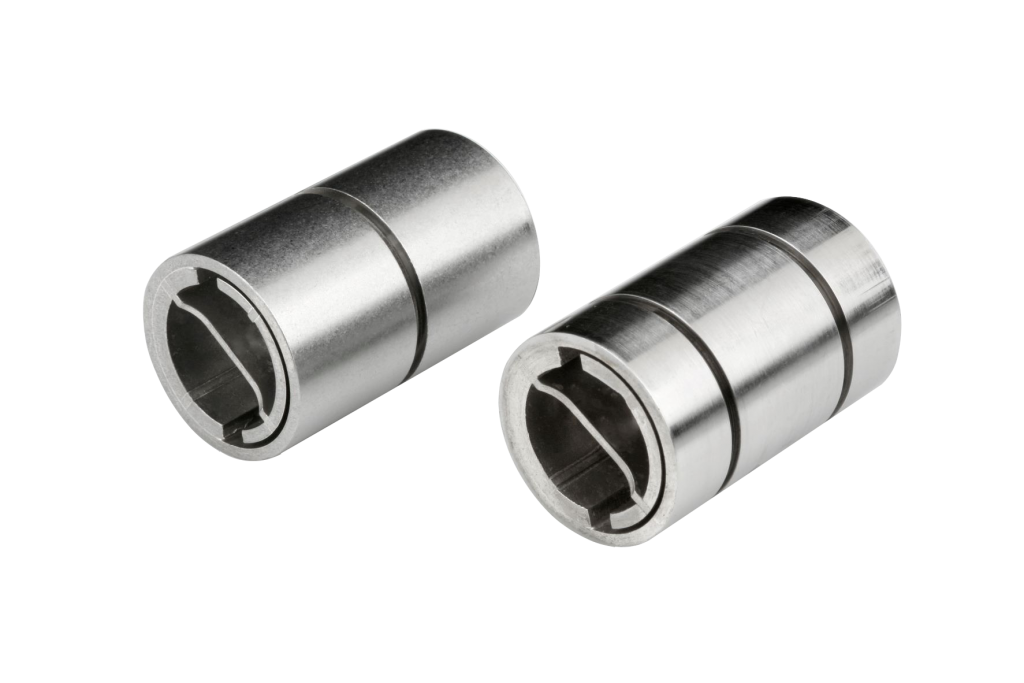
\includegraphics[width=10cm, keepaspectratio]{flexure_pivot}
\caption{The Free-Flex® Pivot Bearing}
\label{flexure-pivot}
\end{center}
\end{figure}

Here are some of the advantages of a rotational flexure over a classical ball bearing.
\begin{itemize}
\item No sliding friction
\item No lubrication needed
\item No backlash
\end{itemize}

Additionally, rotational flexures find applicability in robotics. They can be used as the elastic component in series elastic actuators to implement torque control, which is an economical alternative to field oriented control of BLDC motors.

\section{Quantifying Flexure Quality}
Here we will define a quantitative metric that encodes our intuitive understanding of what makes a good rotational  flexure. 

Let the parameters $p$ encode the geometry of the flexure. For concreteness, assume that we begin with a base finite element mesh with $N$ elements, and $p \in \{0, 1\}^N$, where the bit value $p_i$ determines whether there is material in element $i$ ($p=1$), or whether that element is a void ($p=0$). Given the parameters $p$, we will refer to the resulting candidate flexure as $\Theta_p$.

Now suppose we grab onto a segment of $\Theta_p$ at the outer boundary and prescribe a displacement of this segment through angle $\theta$, say 0.2 radians about the axis of rotation of the flexure, while keeping inner boundary fixed. Figures \ref{before-deformation} and \ref{after-deformation} show such an experiment on a candidate flexure, using the finite element code produced for this project.

\begin{figure}[H]
\begin{center}
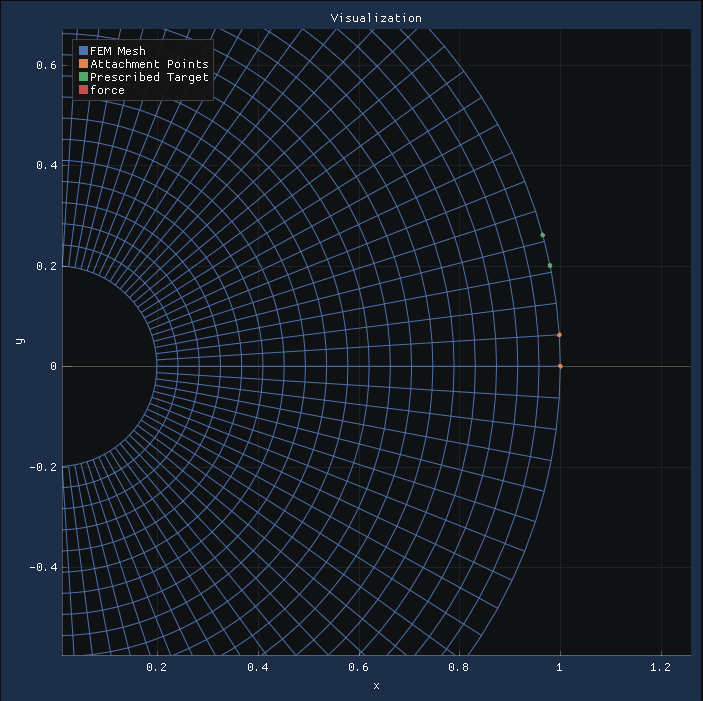
\includegraphics[width=12cm, keepaspectratio]{before_deformation}
\caption{Experiment 1, Undeformed Configuration}
\label{before-deformation}
We are to grab onto the material at the orange markers and forcibly displace them so that they meet the green markers. Note that the green markers are not attached to the material. They simply denote target coordinates in ambient space.
\end{center}
\end{figure}

\begin{figure}[H]
\begin{center}
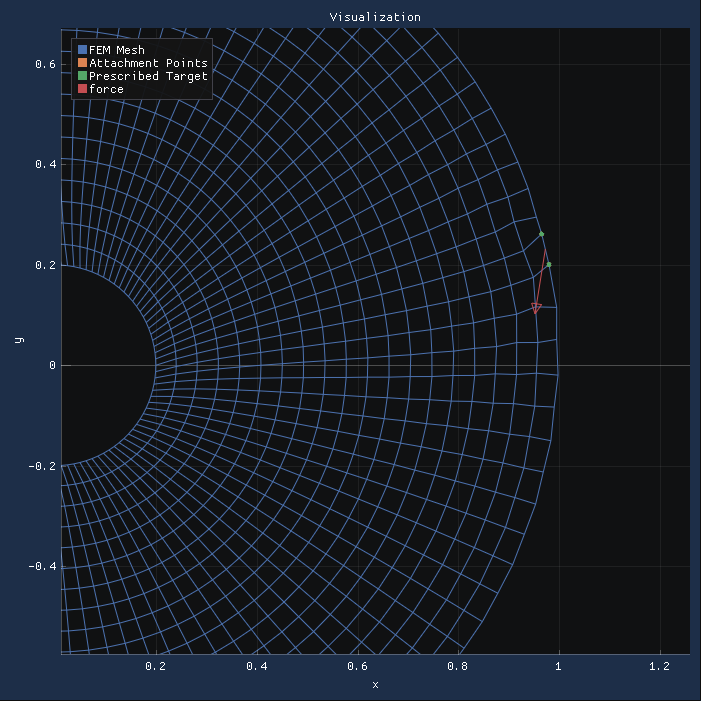
\includegraphics[width=14cm, keepaspectratio]{after_deformation}
\caption{Experiment 1, Deformed Configuration}
\label{after-deformation}
Having forcibly displaced the orange markers, they now coincide with the green markers. The mesh deforms and imposes a reaction force (pink), which attempts to bring the mesh back into its undeformed configuration.
\end{center}
\end{figure}

Figure \ref{after-deformation} shows the reation force arising from the deformation. It's clear that the reaction force is a function of the specified angular displacement $\theta$, and the geometry parameters $p$. So we may write it as $f(p, \theta)$. Note that there is no obstruction to specifying a radial displacement $r$ instead of $\theta$ (see Figures \ref{before-deformation-radial} and \ref{after-deformation-radial}). And we may even prescribe a radial and angular displacement $(r, \theta)$ at the same time, so we write the aforementioned reaction force function as $f(p, r, \theta)$. 

\begin{figure}[H]
\begin{center}
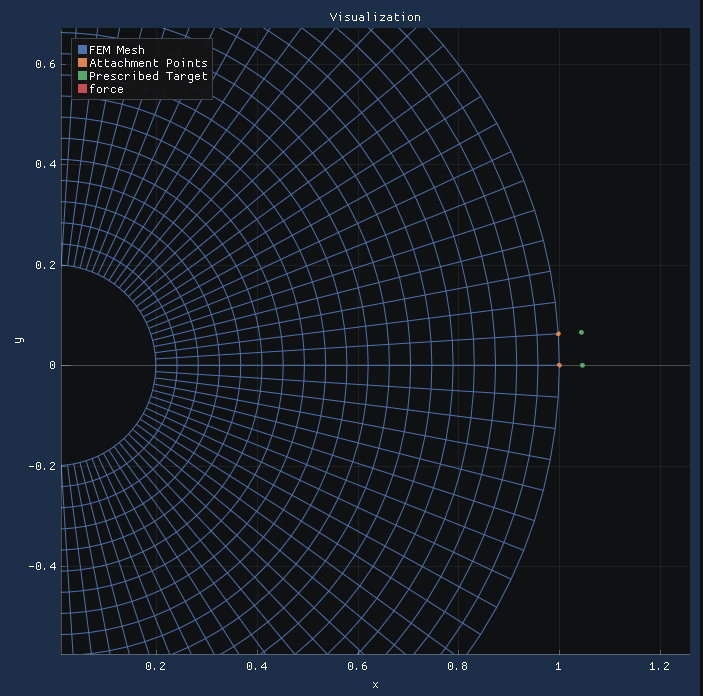
\includegraphics[width=12cm, keepaspectratio]{before_deformation_radial}
\caption{Experiment 2, Undeformed Configuration}
\label{before-deformation-radial}
We are to grab onto the orange markers and forcibly displace them so that they meet the green markers.
\end{center}
\end{figure}

\begin{figure}[H]
\begin{center}
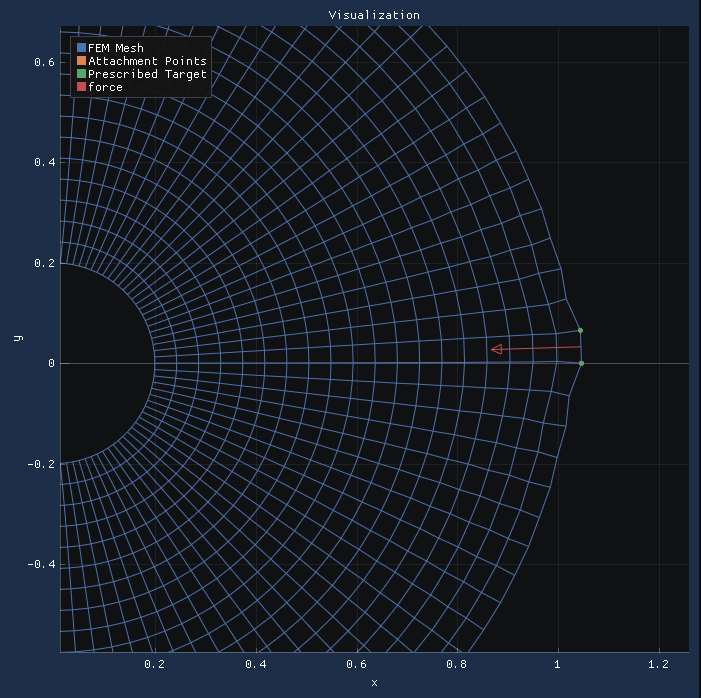
\includegraphics[width=14cm, keepaspectratio]{after_deformation_radial}
\caption{Experimeent 2, Deformed Configuration}
\label{after-deformation-radial}
The resulting deformation and reaction force (pink).
\end{center}
\end{figure}

Now that we have the reaction force function $f(p, r, \theta)$ that arises from the equilibrium solution of a prescribed displacement problem, we are ready to formulate the quality metric for a rotational flexure. First it will be useful to decompose $f$ into its radial and tangential components. Let $n(\theta) := \begin{bmatrix} \cos(\theta) \\ \sin(\theta) \end{bmatrix}$, and $n^\perp(\theta) :=  \begin{bmatrix} -\sin(\theta) \\ \cos(\theta) \end{bmatrix}$. Then define the radial and tangential components of $f$ as follows.
$$f_{\text{R}}(p, r, \theta) := f(p, r, \theta) \cdot n(\theta)$$
$$f_\text{T}(p, r, \theta) := f(p, r, \theta) \cdot n^\perp(\theta)$$

Now consider performing prescribed displacement experiments of the type described in previous section on a classical roller bearing. If we push or pull radially on the bearing, the bearing will push back on us to resist movement from its fixed axis, as it was designed to do. In the perfect rigid body case, $|f_\text{R}(p, r, \theta)| \approx \infty$ when $r \ne 0$. However, if we simply rotate the outer race of the bearing, the bearing will not push or pull radially at all. In other words, $f_\text{R}(p, 0, \theta) \approx 0$.

Using these idealized reaction force profiles as a guide, we define the following flexure quality metric $\phi(p)$ for the flexure with geometry parameters $p$.

$$\phi(p) :=  -\int_{-\pi/6}^{\pi/6} |f_{R}(p, 0, \theta)| d\theta + \int_{-\pi/6}^{\pi/6} |f_{R}(p, - \epsilon, \theta) | d\theta + \int_{-\pi/6}^{\pi/6} |f_{R}(p, \epsilon, \theta)| d\theta$$


In the above expression, the desired angular range of motion is assumed $[-\pi/6, \pi/6]$ although a larger or smaller value can obviously be used. The parameter $\epsilon > 0$ is used to test for reaction forces when pressing and pulling radially on the design. It can be set to some small number, say $\epsilon=0.01$. In implementations, the integral should also be replaced by a finite sum approximation.

The design $p$ is rewarded for having high stiffness in the radial direction when trying to displace the material radially, but punished for producing radial reaction forces when there is only angular displacement. Note that we have not used the tangential reaction force function $f_\text{T}$ yet. We can incorporate this term to promote similarity to a desired angle-torque curve, $\tau(\theta)$. We arrive at the final form of the flexure quality metric.

\[\begin{aligned}
    \phi(p) &:=  -\int_{-\pi/6}^{\pi/6} |f_{R}(p, 0, \theta)| d\theta + \int_{-\pi/6}^{\pi/6} |f_{R}(p, - \epsilon, \theta) | d\theta + \int_{-\pi/6}^{\pi/6} |f_{R}(p, \epsilon, \theta)| d\theta 
- \int_{-\pi/6}^{\pi/6} |\tau(\theta)  - f_T(p, 0, \theta)|d\theta
  \end{aligned}
\]

One then produces a flexure design by seeking $p^* = \argmax_p \phi(p)$. For this project, we will use the genetic algorithm, with genes $p$, and fitness function $\phi(p)$ to produce a flexure design.

There are many trivial modifications that can be made to the flexure quality metric. For example, hyperparameters may be selected to scale each integral. Or the absolute values can be replaced with squares. Or the sign of the radial reaction force $f_\text{R}$ can be taken into account. One can play around with the exact formulation of $\phi(p)$ using the building blocks $f_\text{T}$ and $f_\text{R}$ and see which produces the best results. 

Computation of $\phi$ invoves computing $f$ which entails solving a prescribed displacement static equilibrium finite element problem. So it is now becomes important to understand the details of such a problem.
\newpage

\section{Nonlinear Elasticity}
\paragraph{}
We must use nonlinear elasticity. But first it's useful to understand why the theory of infinitesimal elasticity is not sufficient to model a rotational flexure. Suppose a traction $f$ is prescribed at point on the boundary of the flexure. See figure \ref{prescribed-traction-experiment}, where a rotational flexure is depicted abstractly as an annulus.

\begin{figure}[h!]
\begin{center}
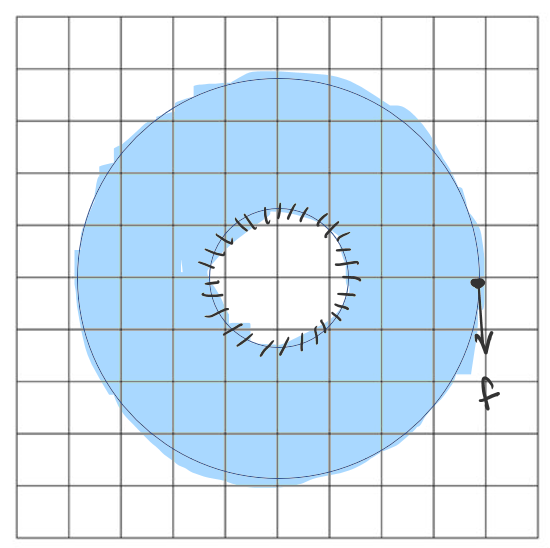
\includegraphics[width=10cm, keepaspectratio]{prescribed_traction_experiment}
\caption{Prescribed traction on a Rotational Flexure}
\label{prescribed-traction-experiment}
\end{center}
\end{figure}

The inner boundary of the annulus is fixed. The material of the flexure is colored solid blue, but should be understood that there may be voids and other complex geometry inside the material such that the flexure rotates as $f$ is increased. Under infinitesimal elasticity, the equilibrium displacements  $u$ turn out to be a linear function of the prescribed traction. So it is clear that, in the linear model, material points will only deform along straight lines as we increase $f$. In the finite elements setting, this is clear from the solution expression $u = K^{-1} f$.

This demonstrates the need to use a nonlinear model of elasticity. One of the simplest such models is the \textbf{St. Venant-Kirchoff} model. The constitutive law is formed by starting from Hooke's Law.
$$ T = \lambda \Tr(\hat E) I + 2 \mu \hat E \;\; \text{(Hooke's Law)}$$

One then simply replaces the infinitesimal strain tensor $\hat{E} = \frac 1 2 (\nabla u + \nabla u^T)$ with the Green-Lagrange strain tensor $E =\frac 1 2 (\nabla u + \nabla u^T + \nabla u^T \nabla u) $, and replacing the stress tensor $T$ with the $ S$, the $2^\text{nd}$ Piola stress tensor.

$$ S = \lambda \Tr(E) I + 2 \mu E \;\; \text{(St. Venant-Kirchoff Law)}$$. In this project, candidate flexures will be analyzed using the St. Venant-Kirchoff constitutive equation above.

\section{Equilibirum Conditions for St. Venant-Kirchoff}
In the finite element setting, the displacement field $U$ is parameterized by  

\end{document}